%
% 4fAufbau.tex -- Bild zum Thema Optische Fouriertransformation <opt>
%
% (c) 2023 Marco Niederberger, Yanick Schoch; OST Ostschweizer Fachhochschule
%

\documentclass[tikz]{standalone}
\usepackage{txfonts}
\usepackage{pgfplots}

\pgfplotsset{compat=1.16}
\def\skala{1}

\begin{document}

\begin{tikzpicture}[>=latex,thick,scale=\skala]
    \node[inner sep=0pt, anchor=west] at (-7,0) {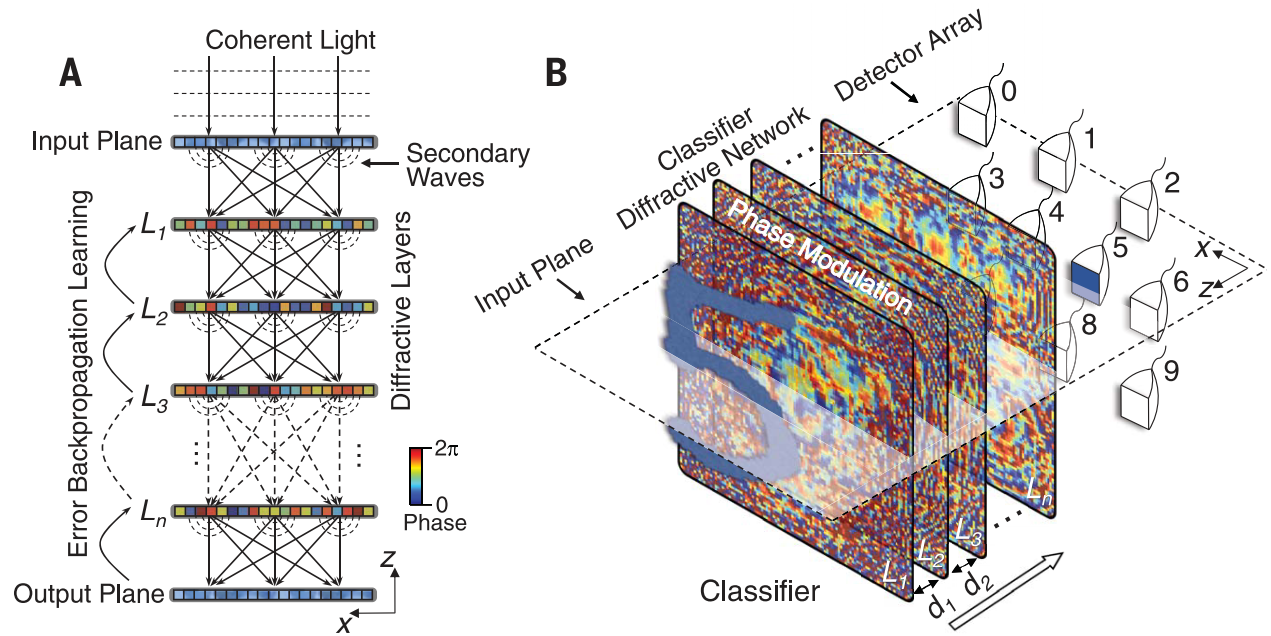
\includegraphics[height=32mm]{handwriting_xing.png}};
    \node[inner sep=0pt, anchor=east] at (3.3,0) {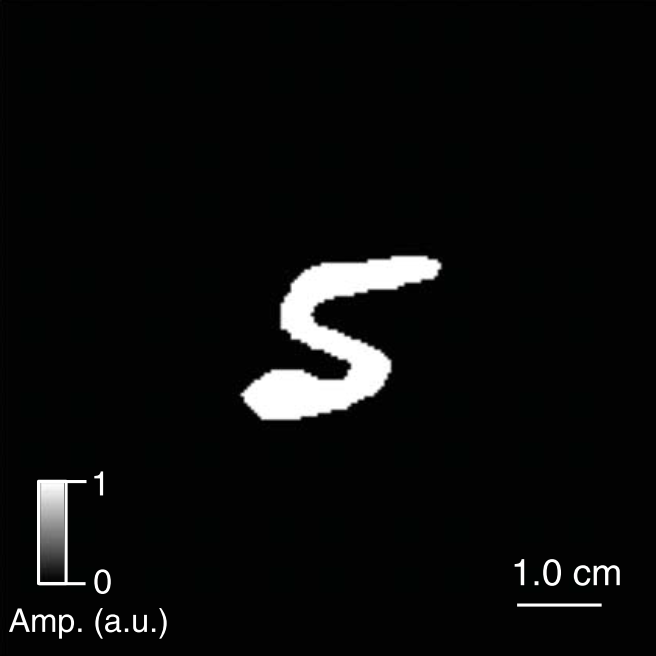
\includegraphics[height=32mm]{handwriting_5_input_xing.png}};
    \node[inner sep=0pt, anchor=east] at (7,0) {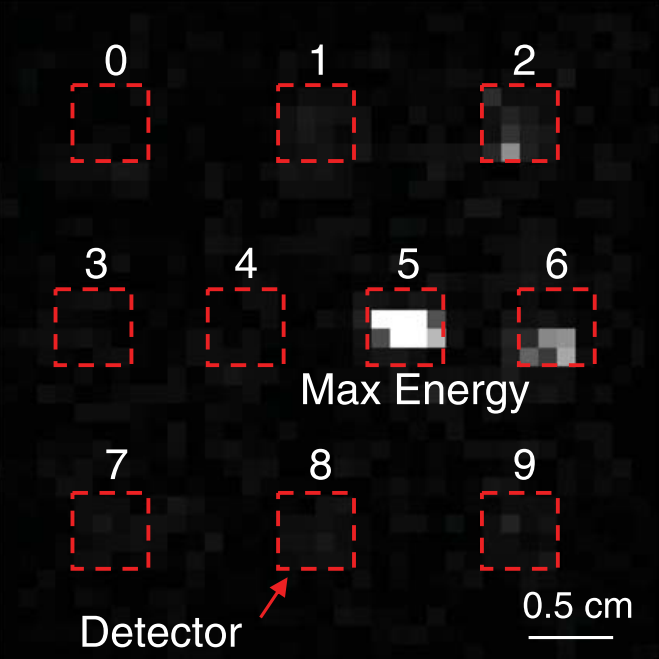
\includegraphics[height=32mm]{handwriting_5_output_xing.png}};

    \node[draw=none] at (-3.8, -2.2) {a) Schematischer Aufbau};
    \node[draw=none] at (1.6, -2.2) {b) Eingang};
    \node[draw=none] at (5.4, -2.2) {c) Ausgang};

\end{tikzpicture}
\end{document}

